\chapter{Analyse, Conception et Architecture}

\begin{spacing}{1.25}
{\large

\section{Choix technologiques}

Le choix de la stack technique a été guidé par trois critères : la rapidité de
développement (délai d'un mois), la maturité des outils (documentation, communauté)
et la sécurité intégrée (pas d'add-ons nécessaires pour les fonctionnalités critiques).

\begin{table}[ht]
\centering
\caption{Comparaison et justification des choix technologiques}
\label{tab:techstack}
\begin{tabularx}{\textwidth}{|l|l|X|}
\hline
\textbf{Couche} & \textbf{Choix retenu} & \textbf{Justification dans le contexte du stage} \\
\hline
Backend & Django + DRF & Stack maîtrisée. L'administration Django et les modules DRF (sérialisation, permissions, pagination) évitent de réimplémenter des fonctionnalités standard, ce qui est décisif sur un délai d'un mois. \\
\hline
Frontend & React.js + Vite & Framework connu, documentation abondante, large choix de composants UI. Le choix est pragmatique : utiliser ce qu'on maîtrise plutôt que d'apprendre un nouveau framework en parallèle du développement. \\
\hline
Base de données & PostgreSQL & Standard de facto avec Django. Support natif du type JSON (utile pour \texttt{AuditLog.changes}) et de \texttt{TIMESTAMPTZ} pour la gestion précise des deadlines. \\
\hline
Authentification & JWT (simplejwt) & Bibliothèque officielle de l'écosystème DRF, intégrable en quelques heures. La solution couvre le besoin (usage interne, une seule organisation) sans nécessiter un serveur OAuth2 dédié, hors scope pour ce stage. \\
\hline
Conteneurisation & Docker Compose & Outil maîtrisé permettant de démarrer les 5 services en une commande. Kubernetes serait pertinent pour un déploiement en production à grande échelle, mais constitue une complexité opérationnelle injustifiée ici. \\
\hline
Proxy & Nginx + HTTPS & Configuration TLS simple et bien documentée. Gunicorn seul ne gère pas le TLS nativement et n'est pas conçu pour être exposé directement. \\
\hline
CI/CD & GitHub Actions & CI gratuite, intégrée au dépôt, sans infrastructure à maintenir. Adapté à un projet solo avec un seul environnement cible. \\
\hline
\end{tabularx}
\end{table}

\paragraph{Django} a été préféré pour son administration intégrée (économie de 3 à 4
jours), son ORM prévenant nativement les injections SQL, et DRF qui fournit
sérialisation, permissions et pagination sans code supplémentaire.

\paragraph{PostgreSQL} offre un support natif des colonnes JSON (utile pour
\texttt{AuditLog.changes}), un type \texttt{TIMESTAMPTZ} précis pour le suivi des
délais, et de meilleures performances sur la recherche textuelle avec l'opérateur
\texttt{ILIKE}.

\paragraph{Docker Compose} permet de démarrer l'ensemble du système (frontend,
backend, base de données, proxy, scheduler) en une seule commande,
garantissant la reproductibilité entre environnements de développement
et de démonstration.

% -------------------------------------------------------------------

\section{Conduite du projet}

\subsection{Méthodologie adoptée}

Face à une contrainte de délai d'un mois et à un périmètre fonctionnel
initialement estimé mais susceptible d'être affiné au fil des retours,
une approche \textbf{Agile adaptée} a été adoptée, s'inspirant du cadre
Scrum tout en tenant compte du contexte d'un développeur solo.

Chaque semaine constituait un sprint d'une durée fixe, avec un livrable
démontrable à la fin. En début de sprint, le backlog était revu et priorisé
en concertation avec les encadrants ; en fin de sprint, une démo informelle
permettait de valider les fonctionnalités réalisées et d'ajuster les priorités
pour le sprint suivant. Le suivi quotidien des tâches a été assuré via un
tableau Kanban personnel organisé en trois colonnes : \textit{À faire},
\textit{En cours}, \textit{Terminé}.

Ce choix a été préféré à une approche cycle en V classique pour deux raisons
principales : la nature incrémentale du projet (chaque sprint livrait une
couche fonctionnelle complète et testable), et la nécessité de faire valider
les choix de sécurité au fur et à mesure plutôt qu'en fin de projet.

% -------------------------------------------------------------------

\subsection{Planification et backlog}

\subsubsection{Backlog produit}

Les fonctionnalités ont été priorisées selon le modèle \textbf{MoSCoW}
(Must-Have, Should-Have, Could-Have), en accord avec les exigences
exprimées par les encadrants en début de stage.

\begin{table}[ht]
\centering
\caption{Backlog produit}
\label{tab:backlog}
\begin{tabularx}{\textwidth}{|l|l|X|c|c|}
\hline
\textbf{ID} & \textbf{Priorité} & \textbf{User Story} & \textbf{Sprint} & \textbf{Statut} \\
\hline
US-01 & Haute & Admin peut créer et gérer les comptes utilisateurs avec rôles & S1 & \checkmark \\
\hline
US-02 & Haute & Utilisateur se connecte via email/mot de passe, reçoit un JWT & S1 & \checkmark \\
\hline
US-03 & Haute & Access token rafraîchi automatiquement via cookie httpOnly & S1 & \checkmark \\
\hline
US-04 & Haute & Manager peut créer un appel d'offres (titre, budget, délais) & S2 & \checkmark \\
\hline
US-05 & Haute & Manager peut publier, clôturer ou attribuer une offre & S2 & \checkmark \\
\hline
US-06 & Moyenne & Analyst peut consulter toutes les offres et évaluer les soumissions & S2 & \checkmark \\
\hline
US-07 & Moyenne & Upload de documents PDF/DOCX associés à une offre & S2 & \checkmark \\
\hline
US-08 & Haute & Contrôle d'accès RBAC appliqué sur tous les endpoints & S3 & \checkmark \\
\hline
US-09 & Haute & Documents financiers chiffrés AES-256-GCM à l'upload & S3 & \checkmark \\
\hline
US-10 & Haute & Journal d'audit enregistrant toutes les opérations d'écriture & S3 & \checkmark \\
\hline
US-11 & Moyenne & Notifications automatiques générées avant expiration des délais & S3 & \checkmark \\
\hline
US-12 & Haute & Société externe soumet une offre via portail public sans compte & S4 & \checkmark \\
\hline
US-13 & Moyenne & Export PDF d'un rapport de synthèse par offre & S4 & \checkmark \\
\hline
US-14 & Moyenne & Pipeline CI (lint flake8 + pytest) déclenché à chaque push & S4 & \checkmark \\
\hline
\end{tabularx}
\end{table}

\subsubsection{Diagramme de Gantt}

\begin{figure}[ht]
\centering
\fbox{%
  \begin{minipage}{0.92\textwidth}
    \vspace{3.5cm}
    \centering
    \textit{[Diagramme de Gantt -- à insérer]}
    \vspace{3.5cm}
  \end{minipage}%
}
\caption{Diagramme de Gantt du projet (6 août -- 6 septembre 2025)}
\label{fig:gantt}
\end{figure}

% -------------------------------------------------------------------

\subsection{Déroulement des sprints}

Le projet a été découpé en quatre sprints hebdomadaires, chacun centré sur un
objectif livrable.

\begin{description}
    \item[Sprint 1 (6--12 août)] Fondations : Docker Compose, Django, PostgreSQL,
    authentification JWT, modèle User avec rôles.
    Livrable : connexion fonctionnelle, endpoints auth testés via Postman.

    \item[Sprint 2 (13--19 août)] Fonctionnalités métier : offres, candidats,
    soumissions, frontend React connecté à l'API, upload de documents.
    Livrable : un manager peut créer une offre, enregistrer des soumissions.

    \item[Sprint 3 (20--26 août)] Sécurité et notifications : RBAC, journal d'audit,
    monitoring des délais, chiffrement AES-256-GCM, notifications en application.
    Livrable : rôles appliqués, documents sensibles chiffrés, alertes actives.

    \item[Sprint 4 (27 août -- 6 septembre)] Portail public, rapports PDF,
    tests, pipeline CI, documentation.
    Livrable : application complète, testée, déployable en une commande.
\end{description}

\subsubsection{Bilan des sprints}

\textbf{Sprint 1.} La configuration du réseau Docker (communication inter-conteneurs,
variables d'environnement) a pris plus de temps qu'estimé. La configuration du
cookie httpOnly pour le refresh token a nécessité une phase de recherche sur
la gestion des cookies cross-origin avec DRF. Le livrable a été atteint avec
un jour de retard, récupéré en début de Sprint 2.

\textbf{Sprint 2.} La complexité de l'upload de documents (validation MIME,
gestion des fichiers Django) a conduit à différer le chiffrement AES au Sprint 3,
où il a été intégré naturellement avec les autres fonctionnalités de sécurité.
Les fonctionnalités métier principales ont été livrées dans les délais.

\textbf{Sprint 3.} L'intégration d'AES-256-GCM a nécessité une journée de
recherche non planifiée sur la bibliothèque \texttt{cryptography} (gestion
du nonce, format de stockage). Le scheduler de monitoring des délais a été
simplifié : une boucle shell dans un conteneur dédié plutôt qu'une intégration
Celery, jugée trop complexe pour le délai disponible.

\textbf{Sprint 4.} La configuration du pipeline GitHub Actions (base PostgreSQL
de test, variables d'environnement CI) a été le dernier élément ajouté,
achevé dans les deux derniers jours du stage. La documentation et le script
de démonstration \texttt{seed\_demo.py} ont été finalisés en parallèle.

% -------------------------------------------------------------------

\subsection{Gestion des risques}

\begin{table}[ht]
\centering
\caption{Registre des risques du projet}
\label{tab:risques}
\begin{tabularx}{\textwidth}{|X|c|c|p{5cm}|}
\hline
\textbf{Risque} & \textbf{Probabilité} & \textbf{Impact} & \textbf{Stratégie de mitigation} \\
\hline
Mauvaise estimation de la durée d'une fonctionnalité complexe
& Moyenne & Élevé
& Timeboxing strict de 2 jours par sous-tâche ; descope vers le sprint suivant si dépassé \\
\hline
Instabilité d'une bibliothèque tierce (ex. simplejwt, cryptography)
& Faible & Moyen
& Vérification des versions LTS et activité des dépôts avant adoption \\
\hline
Perte du code source (panne matérielle, suppression accidentelle)
& Faible & Critique
& Dépôt Git privé avec push quotidien, branches de sauvegarde hebdomadaires \\
\hline
Évolution du périmètre fonctionnel en cours de sprint
& Moyenne & Moyen
& Validation du backlog avec le maître de stage en début de chaque sprint \\
\hline
Incompatibilité entre services Docker (version PostgreSQL, réseau)
& Faible & Élevé
& Tests d'intégration dès le Sprint 1 ; health checks sur tous les services \\
\hline
\end{tabularx}
\end{table}


% -------------------------------------------------------------------

\section{Modélisation des besoins}

\subsection{Diagramme de cas d'utilisation}

\begin{figure}[ht]
\centering
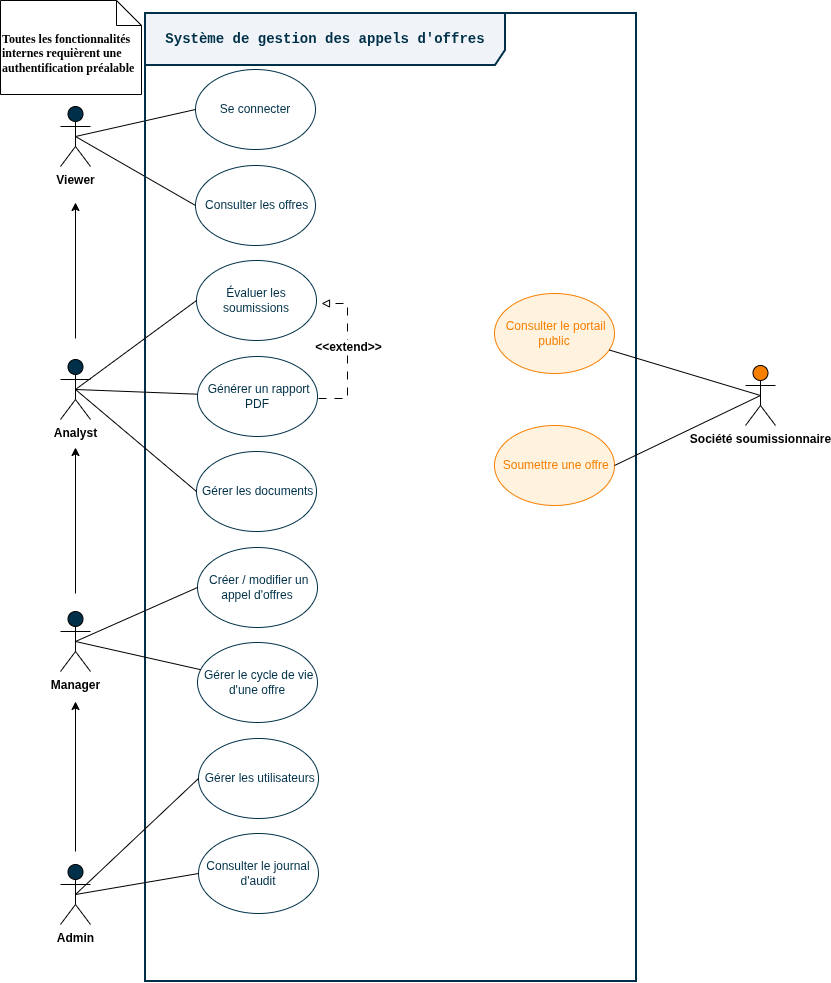
\includegraphics[width=0.9\textwidth]{images/use_case.png}
\caption{Diagramme de cas d'utilisation}
\label{fig:usecase}
\end{figure}

Le diagramme de cas d'utilisation (figure~\ref{fig:usecase}) présente les interactions
entre les cinq acteurs du système et les fonctionnalités exposées.
Les acteurs internes (Admin, Manager, Analyst, Viewer) s'authentifient via JWT.
L'acteur externe (Société soumissionnaire) accède uniquement au portail public
sans authentification.

\subsection{Diagramme d'activité -- Cycle de vie d'une offre}

\begin{figure}[ht]
\centering
\fbox{%
  \begin{minipage}{0.85\textwidth}
    \vspace{2cm}
    \centering
    \textit{[À INSÉRER — Diagramme d'activité : cycle de vie d'une offre — renommer activity\_diagram.drawio.png en activity\_lifecycle.png]}
    \vspace{2cm}
  \end{minipage}%
}
\caption{Diagramme d'activité : cycle de vie d'une offre}
\label{fig:activity}
\end{figure}

Le cycle de vie d'une offre est contrôlé côté serveur par la méthode
\texttt{can\_transition\_to()} du modèle \texttt{OfferCall}. Les transitions
autorisées sont :

\[
\text{DRAFT} \rightarrow \text{PUBLISHED} \rightarrow \text{EVALUATION}
\rightarrow \text{AWARDED}
\]

À tout moment avant attribution, une offre peut être annulée (\texttt{CANCELLED})
via l'endpoint \texttt{POST /api/offers/\{id\}/cancel/}. Toute tentative de
transition non autorisée retourne une erreur HTTP 400.

% -------------------------------------------------------------------

\section{Architecture de la solution}

\subsection{Vue globale}

L'application repose sur une architecture \textbf{monolithe modulaire} :
un seul processus Django contenant huit applications indépendantes, déployé
derrière un proxy Nginx gérant le TLS.

\begin{figure}[ht]
\centering
\fbox{%
  \begin{minipage}{0.85\textwidth}
    \vspace{2cm}
    \centering
    \textit{[À INSÉRER — Architecture globale du système — exporter vers images/architecture.png]}
    \vspace{2cm}
  \end{minipage}%
}
\caption{Architecture globale du système}
\label{fig:architecture}
\end{figure}

Le flux d'une requête authentifiée :

\begin{enumerate}
    \item Le navigateur envoie la requête HTTPS sur le port 443.
    \item Nginx termine le TLS et route vers le frontend React (assets statiques)
    ou vers le backend Django (\texttt{/api/*}).
    \item Django traite la requête : authentification JWT, vérification du rôle,
    logique métier, accès PostgreSQL via l'ORM.
    \item La réponse remonte par Nginx vers le client.
\end{enumerate}

\subsection{Monolithe modulaire vs microservices}

Une architecture microservices aurait nécessité : API gateway, découverte de services,
authentification inter-services, traçage distribué -- impossible à développer seul
en un mois. Le monolithe modulaire offre la séparation des responsabilités via les
frontières des applications Django (chaque app possède ses propres \texttt{models.py},
\texttt{views.py}, \texttt{serializers.py}, \texttt{urls.py}), tout en conservant
la simplicité opérationnelle (\texttt{docker-compose up}).

\subsection{Services Docker Compose}

\begin{table}[ht]
\centering
\caption{Services Docker Compose}
\label{tab:docker-services}
\begin{tabularx}{\textwidth}{|l|l|X|}
\hline
\textbf{Service} & \textbf{Port} & \textbf{Rôle} \\
\hline
\texttt{db} & 5432 & PostgreSQL, données persistées sur volume nommé \\
\hline
\texttt{backend} & 8000 & Django + Gunicorn, migrations automatiques au démarrage \\
\hline
\texttt{frontend} & 3000 & React SPA (build statique ou serveur de dev) \\
\hline
\texttt{nginx} & 80, 443 & Proxy inverse, terminaison TLS, redirection HTTP→HTTPS \\
\hline
\texttt{scheduler} & -- & Boucle \texttt{check\_deadlines \&\& sleep 3600} \\
\hline
\end{tabularx}
\end{table}

Tous les services disposent de vérifications de santé (\textit{health checks}).
Les services \texttt{backend} et \texttt{nginx} démarrent uniquement après
que \texttt{db} soit déclaré sain (\texttt{condition: service\_healthy}).

% -------------------------------------------------------------------

\section{Conception détaillée}

\subsection{Modèle de données}

Le modèle de données comprend sept entités principales,
représentées dans le diagramme entité-relation (figure~\ref{fig:erd}).

\begin{figure}[ht]
\centering
\fbox{%
  \begin{minipage}{0.85\textwidth}
    \vspace{2cm}
    \centering
    \textit{[À INSÉRER — Diagramme entité-relation — exporter vers images/erd.png]}
    \vspace{2cm}
  \end{minipage}%
}
\caption{Diagramme entité-relation}
\label{fig:erd}
\end{figure}

Les choix de conception notables sont :

\begin{description}
    \item[UUID comme clé primaire] Tous les modèles utilisent \texttt{UUIDField}
    comme clé primaire. Contrairement aux entiers auto-incrémentés, les UUIDs
    ne révèlent pas le volume de données et empêchent l'énumération
    (\texttt{/offers/1}, \texttt{/offers/2}).

    \item[\texttt{uploaded\_by} nullable] Le champ \texttt{Document.uploaded\_by}
    est nullable avec \texttt{on\_delete=SET\_NULL}. Les documents déposés via
    le portail public (sans compte utilisateur) ont ce champ à \texttt{NULL}.
    Les documents uploadés par le personnel ont leur auteur référencé.

    \item[Deadlines séparées] \texttt{OfferCall} possède deux champs distincts :
    \texttt{submission\_deadline} (date limite de dépôt pour les candidats) et
    \texttt{evaluation\_deadline} (date limite d'évaluation pour les équipes internes).
    Le scheduler surveille les deux indépendamment.

    \item[\texttt{AuditLog.changes} en JSON] Le champ \texttt{changes} stocke un
    objet JSON arbitraire représentant les modifications apportées à la ressource.
    Cette approche évite une table de colonnes rigides et s'adapte à n'importe
    quelle ressource auditée.
\end{description}

\subsection{Conception de l'API REST}

L'API respecte les conventions REST : ressources nommées, méthodes HTTP sémantiques,
codes de retour standard. La pagination est systématique sur les listes
(\texttt{count, next, previous, results}).

\begin{table}[ht]
\centering
\caption{Principaux endpoints de l'API}
\label{tab:api}
\begin{tabularx}{\textwidth}{|l|l|X|}
\hline
\textbf{Endpoint} & \textbf{Méthode} & \textbf{Description} \\
\hline
\texttt{/api/auth/login/} & POST & Connexion, retourne access token + cookie httpOnly \\
\hline
\texttt{/api/auth/refresh/} & POST & Rafraîchit l'access token via le cookie \\
\hline
\texttt{/api/auth/logout/} & POST & Blackliste le refresh token, supprime le cookie \\
\hline
\texttt{/api/offers/} & GET, POST & Liste paginée, création d'offre \\
\hline
\texttt{/api/offers/\{id\}/} & GET, PATCH & Détail, modification \\
\hline
\texttt{/api/offers/\{id\}/publish/} & POST & DRAFT → PUBLISHED \\
\hline
\texttt{/api/offers/\{id\}/close/} & POST & PUBLISHED → EVALUATION \\
\hline
\texttt{/api/offers/\{id\}/award/} & POST & EVALUATION → AWARDED \\
\hline
\texttt{/api/offers/\{id\}/cancel/} & POST & Annulation (tout statut non terminal) \\
\hline
\texttt{/api/documents/upload/} & POST & Upload multipart, chiffrement optionnel \\
\hline
\texttt{/api/documents/\{id\}/download/} & GET & Téléchargement (déchiffrement transparent) \\
\hline
\texttt{/api/notifications/unread-count/} & GET & Nombre de notifications non lues \\
\hline
\texttt{/api/reports/offers/\{id\}/export/} & GET & Export PDF d'une offre \\
\hline
\texttt{/api/audit/logs/} & GET & Journal d'audit (ADMIN uniquement) \\
\hline
\texttt{/api/portal/offers/} & GET & Offres publiées (AllowAny) \\
\hline
\texttt{/api/portal/offers/\{id\}/submit/} & POST & Soumission publique (AllowAny, rate limited) \\
\hline
\end{tabularx}
\end{table}

Les transitions d'état sont des endpoints POST dédiés (et non une modification PATCH
du champ \texttt{status}). Cela garantit que la logique de validation de la transition
est toujours exécutée côté serveur, quelle que soit la requête entrante.

\subsection{Architecture de sécurité}

\subsubsection{Authentification JWT}

Le schéma d'authentification repose sur deux tokens aux durées de vie différentes :
l'access token (15 minutes) et le refresh token (7 jours).

\begin{figure}[ht]
\centering
\fbox{%
  \begin{minipage}{0.85\textwidth}
    \vspace{2cm}
    \centering
    \textit{[À INSÉRER — Diagramme de séquence : flux d'authentification — exporter vers images/seq\_login.png]}
    \vspace{2cm}
  \end{minipage}%
}
\caption{Diagramme de séquence : flux d'authentification}
\label{fig:seqlogin}
\end{figure}

L'access token est stocké en \textbf{mémoire React} (variable d'état dans
\texttt{AuthContext}). Ce choix est délibéré : stocker le token dans
\texttt{localStorage} l'exposerait aux attaques XSS, une vulnérabilité classique
du top 10 OWASP. Un script malveillant injecté dans la page pourrait lire
\texttt{localStorage} mais ne peut pas accéder à une variable JavaScript en mémoire
appartenant à un autre contexte.

Le refresh token est stocké dans un cookie avec les attributs \texttt{HttpOnly},
\texttt{Secure}, \texttt{SameSite=Lax} et \texttt{path=/api/auth/}. L'attribut
\texttt{HttpOnly} empêche tout accès JavaScript au cookie. L'attribut
\texttt{path=/api/auth/} restreint l'envoi du cookie aux seules URLs
\texttt{/api/auth/refresh/} et \texttt{/api/auth/logout/}, évitant qu'il
soit transmis sur les requêtes du portail public.

Au chargement de l'application, un appel silencieux à \texttt{/api/auth/refresh/}
restaure l'access token depuis le cookie, permettant à l'utilisateur de rester
connecté sans ressaisir ses identifiants.

\subsubsection{Contrôle d'accès basé sur les rôles (RBAC)}

Chaque endpoint Django est protégé par une classe de permission DRF :

\begin{table}[ht]
\centering
\caption{Matrice de contrôle d'accès}
\label{tab:rbac}
\begin{tabularx}{\textwidth}{|X|c|c|c|c|}
\hline
\textbf{Action} & \textbf{ADMIN} & \textbf{MANAGER} & \textbf{ANALYST} & \textbf{VIEWER} \\
\hline
Créer une offre & \checkmark & \checkmark & & \\
\hline
Modifier une offre & \checkmark & \checkmark & & \\
\hline
Voir toutes les offres & \checkmark & \checkmark & \checkmark & \\
\hline
Voir offres publiées & \checkmark & \checkmark & \checkmark & \checkmark \\
\hline
Scorer une soumission & \checkmark & \checkmark & \checkmark & \\
\hline
Exporter PDF & \checkmark & \checkmark & \checkmark & \\
\hline
Gérer les utilisateurs & \checkmark & & & \\
\hline
Consulter l'audit log & \checkmark & & & \\
\hline
\end{tabularx}
\end{table}

\subsubsection{Chiffrement AES-256-GCM}

Le chiffrement est appliqué \textbf{sélectivement} aux documents marqués sensibles
(propositions financières, contrats). Le chiffrement de tous les fichiers ajouterait
une latence inutile sur les pièces jointes anodines.

L'algorithme AES-256-GCM (mode Galois/Counter Mode) garantit simultanément :
\begin{itemize}
    \item \textbf{La confidentialité} : les données en clair sont inaccessibles
    sans la clé de 256 bits.
    \item \textbf{L'intégrité} : le tag d'authentification de 128 bits détecte
    toute modification du fichier chiffré.
\end{itemize}

Pour chaque fichier chiffré, un nonce de 12 octets est généré aléatoirement.
Le fichier stocké sur disque contient la concaténation : \texttt{nonce (12B) ||
ciphertext || tag (16B)}. La clé de chiffrement (32 octets = 256 bits) est fournie
via la variable d'environnement \texttt{DOCUMENT\_ENCRYPTION\_KEY} et n'apparaît
jamais dans le code source ni dans le dépôt Git.

\subsubsection{Diagramme de séquence -- Soumission portail public}

\begin{figure}[ht]
\centering
\fbox{%
  \begin{minipage}{0.85\textwidth}
    \vspace{2cm}
    \centering
    \textit{[À INSÉRER — Diagramme de séquence : soumission portail public — exporter vers images/seq\_portal.png]}
    \vspace{2cm}
  \end{minipage}%
}
\caption{Diagramme de séquence : soumission portail public}
\label{fig:seqportal}
\end{figure}

La soumission via le portail public suit un flux en sept étapes :
vérification de l'offre (statut PUBLISHED), contrôle de la deadline, validation
des données, création ou récupération du candidat (upsert par email), vérification
d'unicité, création de la soumission, upload du document, et notification
du responsable assigné.

Ce flux est atomique : en cas d'erreur à l'étape 7 (validation du fichier),
la soumission créée est supprimée pour maintenir la cohérence de la base de données.


}
\end{spacing}

\newpage
